
% this file is called up by thesis.tex
% content in this file will be fed into the main document

%: ----------------------- introduction file header -----------------------
\chapter{Future Work and Conclusions}

% the code below specifies where the figures are stored
\ifpdf
    \graphicspath{{11_future_work_and_conclusions/figures/PNG/}{11_future_work_and_conclusions/figures/PDF/}{11_future_work_and_conclusions/figures/}}
\else
    \graphicspath{{11_future_work_and_conclusions/figures/EPS/}{11_future_work_and_conclusions/figures/}}
\fi

% ----------------------------------------------------------------------
%: ------------------------------- content ----------------------------- 
% ----------------------------------------------------------------------

\section{Commercial Activity in the Field of Social-Network-Based Event Summarization}

The research fields of event summarization and event archiving
based on social network multimedia data have resulted in 
interesting business creations in recent months.
Albeit similarities to our work exist,
there are still many differences in the details.

\paragraph{Mahaya}
 
The company Mahaya has launched a~beta-version
of a~commercial automatic event archiving tool called Seen,
which, based on manually entered event metadata like event name,
location, and dates, uses a~necessarily provided Twitter hashtag
to create a~complete permanent archive of all event-related tweets,
media items, and slide decks.
Based on term frequency and co-occurrence analyses,
the event is split into subevents
and each subevent's hot topics are tried to be detected.
The application's main data source is Twitter,
links to certain media hosting platforms are followed.
Seen does not deduplicate and cluster
similar media items.
A~screenshot of Seen can be found in \autoref{fig:seen}.

\begin{figure}
  \centering
  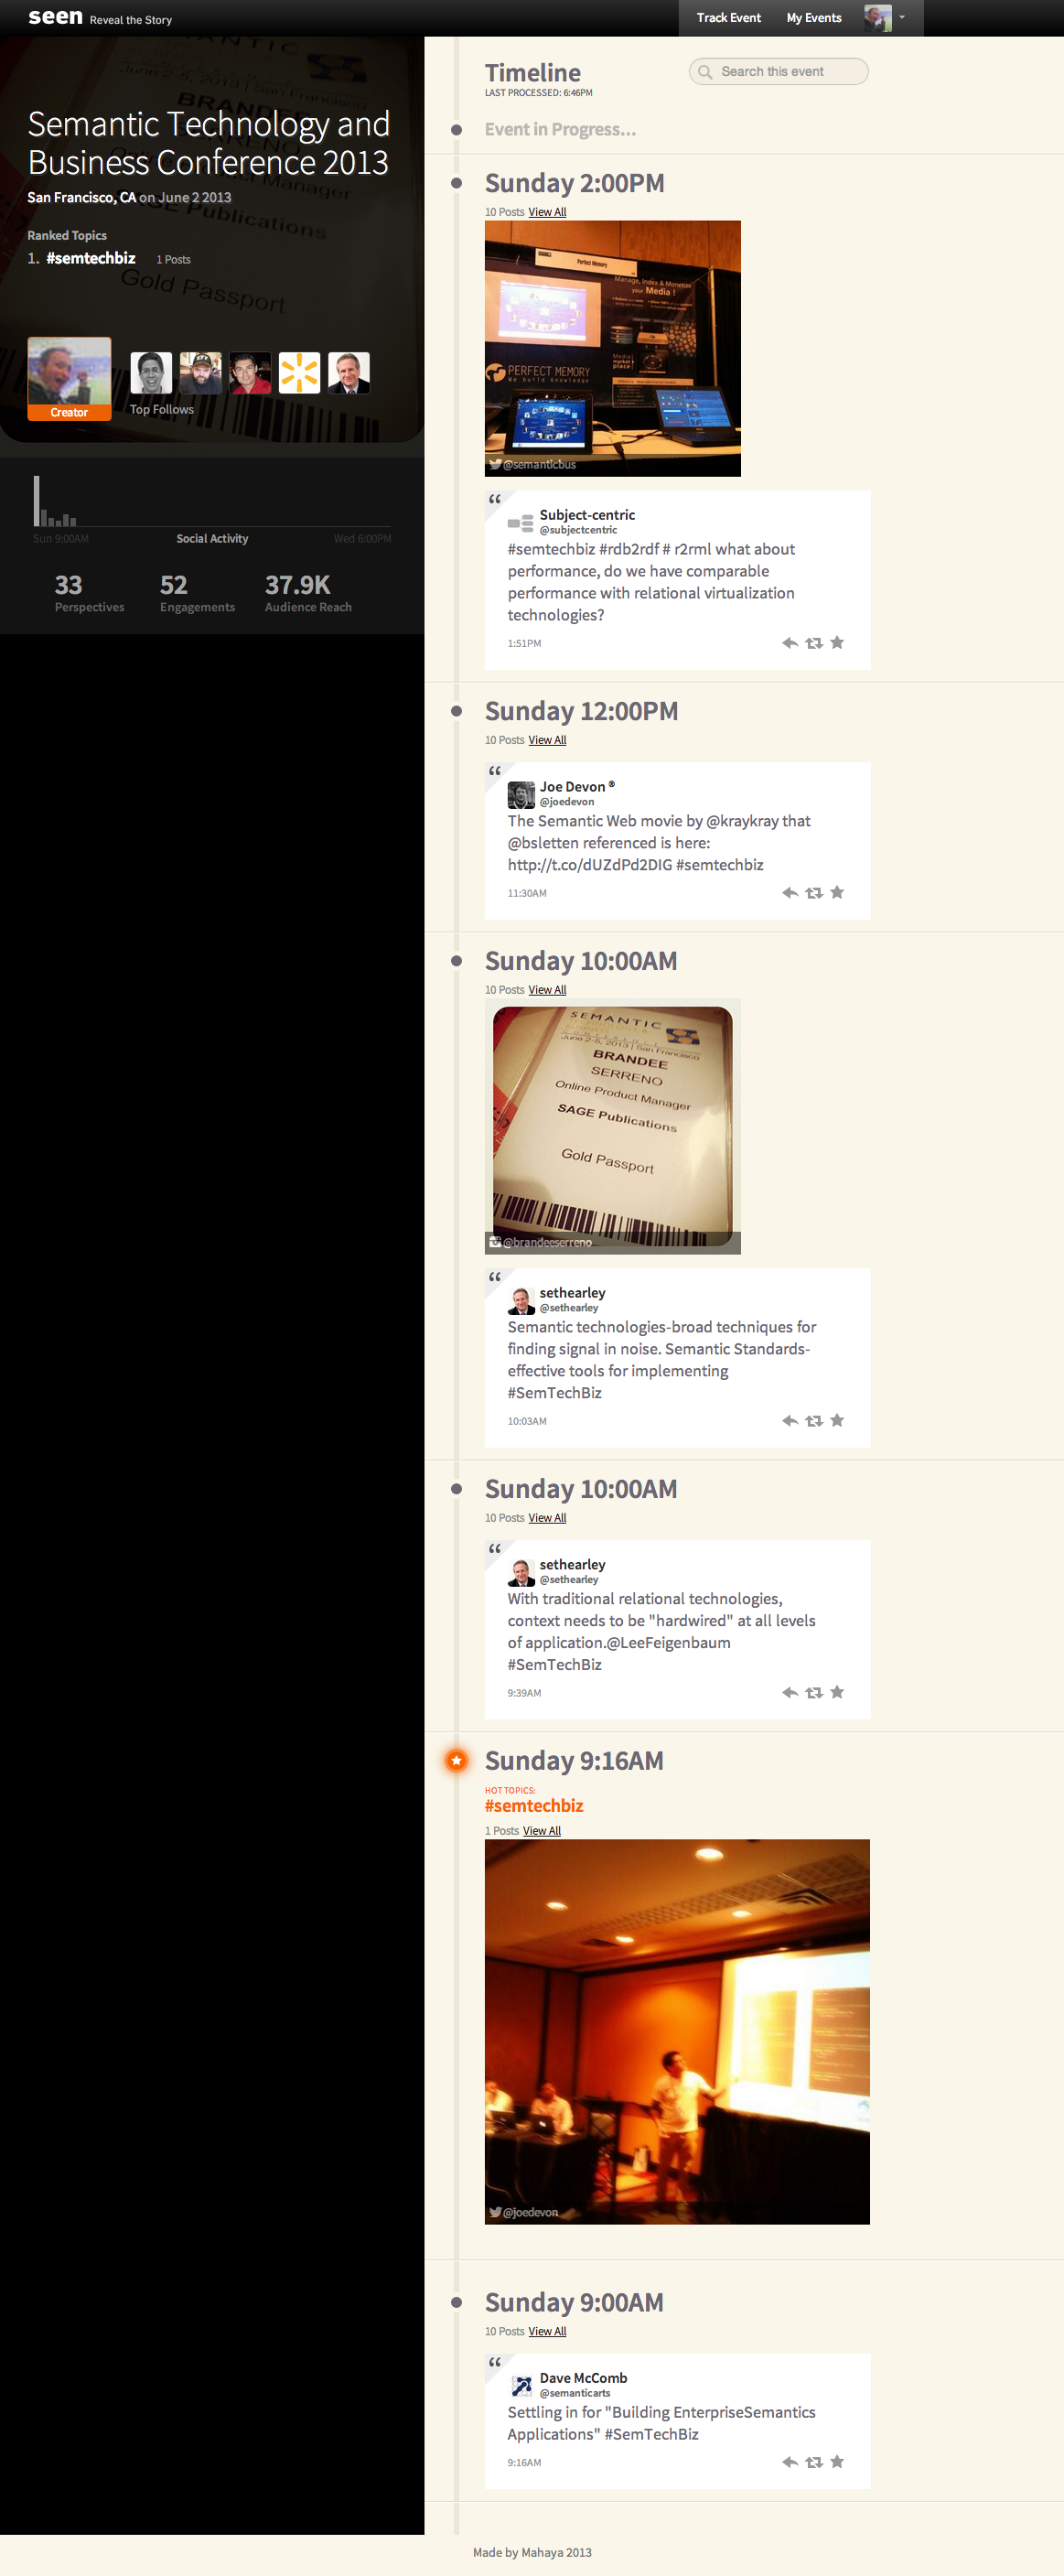
\includegraphics[width=\linewidth]{seen.png}
  \caption{Mahaya's commercial automatic event archiving tool Seen
    (\url{http://mahaya.co/})}
  \label{fig:seen}
\end{figure}

\paragraph{Eventifier}

Eventifier is a~commercial tool that facilitates the automatic permanent archiving of events
in form of event-related photos, videos, tweets, slide decks, 
and event contributors.
Similar to Mahaya's product Seen,
the application's main data source is Twitter.
The manually entered event's official hashtag and potentially existing
official Twitter account serve to encounter event-related content.
Eventifier does not deduplicate and cluster
similar media items.
A~screenshot of Eventifier can be seen in \autoref{fig:eventifier}.

\begin{figure}
  \centering
  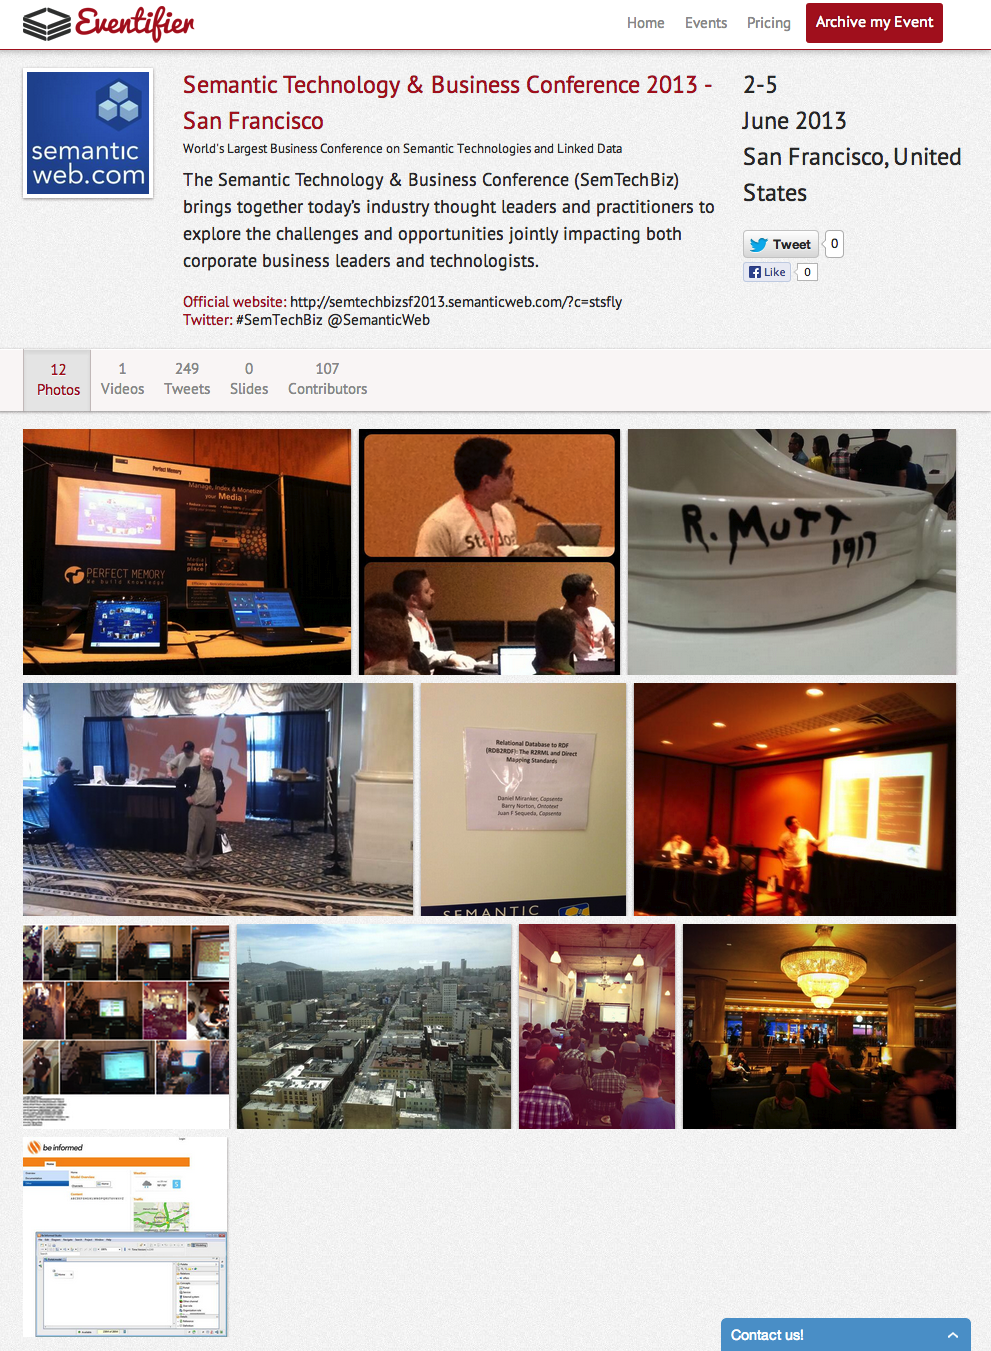
\includegraphics[width=\linewidth]{eventifier.png}
  \caption{The automatic commercial event archiving tool Eventifier
    (\url{http://eventifier.co/})}
  \label{fig:eventifier}
\end{figure}

\paragraph{Storify}

The commercial tool Storify allows for the manual compilation of
event-related media items, articles, and microposts
to generated permanently available stories
that---depending on the level of human curation---%
can efficiently summarize an event.
Storify does not deduplicate and cluster
similar media items.
A~screenshot of Storify can be seen in \autoref{fig:storify}.

\begin{figure}
  \centering
  \includegraphics[width=\linewidth]{storify.png}
  \caption{The manual assisted commercial event archiving tool Storify
    (\url{http://storify.com/})}
  \label{fig:storify}
\end{figure}

\paragraph{Media Finder}

Media Finder is an academic non-commercial tool that
has advanced named entity centric clustering capabilities
based on extracted named entities in microposts.
Media items can be clustered by topic, named entity,
named entity type, and micropost instance.
We have contributed the application's media extraction component,
in consequence the covered social networks
are exactly as described in \autoref{cha:media-item-extraction}.
A~screenshot of Media Finder can be seen in \autoref{fig:mediafinder}.

\begin{figure}
  \centering
  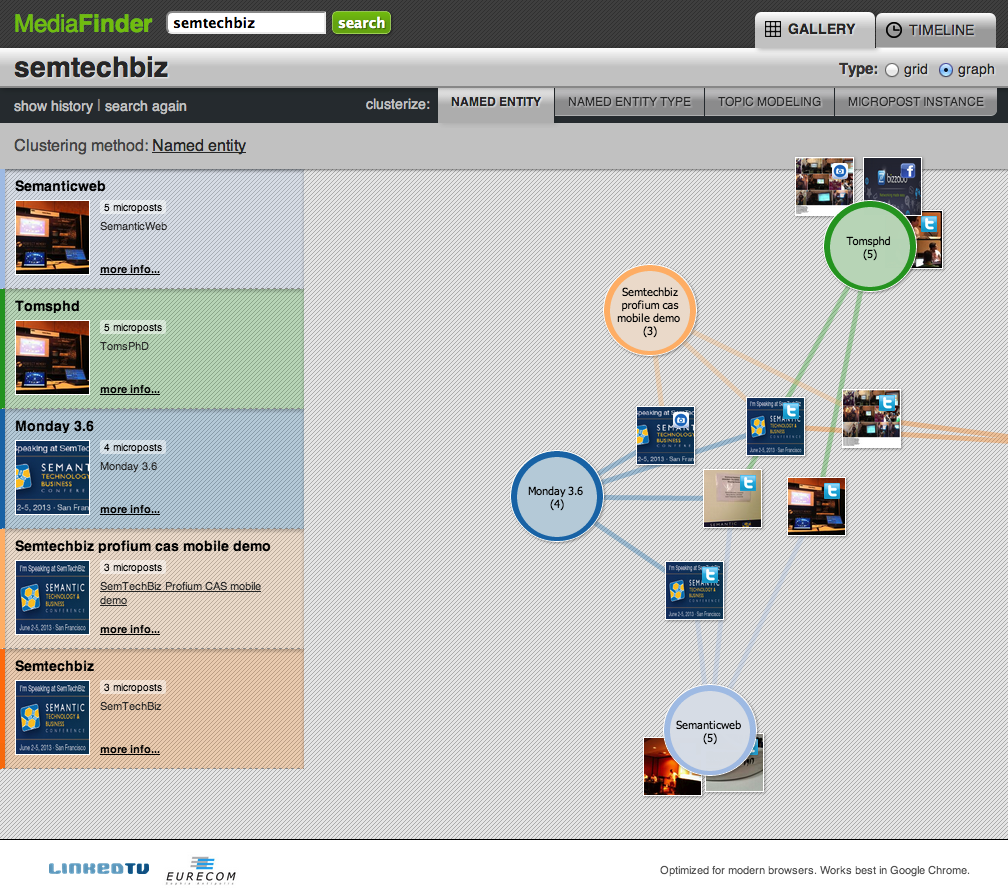
\includegraphics[width=\linewidth]{mediafinder.png}
  \caption{The academic event summarization tool Media Finder}
  \label{fig:mediafinder}
\end{figure}

\subsection{Comparison of Tools}

In the previous paragraphs, we have characterized
commercial and non-commercial tools for the tasks
of event summarization and event archiving. 
\autoref{table:toolcomparison} shows how these tools
compare against our own application Social Media Illustrator,
which, for reference, is depicted again in \autoref{fig:socialmediaillustrator}.
The unique selling point of our application
are its interactive media galleries that together with speech synthesis
as outlined in \autoref{sec:interactivemediagalleries}
allow for truly one of its kind experience when it comes to 
event summary consumption.

\begin{figure}
  \centering
  
\includegraphics[width=\linewidth]{socialmediaillustrator.png}
  \caption{Our own academic event summarization tool Social Media Illustrator}
  \label{fig:socialmediaillustrator}
\end{figure}

\begin{sidewaystable}[h!]
  \centering
  \small
  \begin{tabular}{|l|l|l|l|l|l|}
    \hline
        \backslashbox{\textbf{Property}}{\textbf{Tool}} & \textbf{Seen} & \textbf{Eventifier} & \textbf{Storify} & \textbf{Media Finder} & \textbf{Social Media Illustrator}\\ \hline
      \hline
      \textbf{Data source} & Twitter & Twitter & Multiple & Multiple & Multiple\\
      \textbf{Main task} & Archiving & Archiving & Summarization & Summarization & Summarization\\
      \textbf{Operation mode} & Automatic & Automatic & Manual & Semi-automatic & Semi-automatic\\
      \textbf{Linkable} & Yes & Yes & Yes & Yes & No\\
      \textbf{Downloadable} & No & No & No & No & Yes\\
      \textbf{Customizable} & No & No & Yes & Yes & Yes\\
      \textbf{Interactive} & No & No & No & No & Yes\\
      \textbf{Commercial} & Yes & Yes & Yes & No & No\\
      \hline
    \end{tabular}
    \caption[Comparison of event archiving and summarization tools]{Comparison of commercial and non-commercial event archiving and summarization tools \todo{Check final orientation}}
  \label{table:toolcomparison}
\end{sidewaystable}




\section{Future Research Directions}

\subsection{Media Item Verification}

An aspect that we have left aside so far is the verification
of the credibility and authenticity of both sources
and media items themselves that get shared on social networks.
The growing importance of first-hand eye witness social media in news coverage---%
or even social media being \emph{the} actual news,
as to some extent it was the case with the Boston Bombings%
\footnote{\url{http://en.wikipedia.org/wiki/Boston_Marathon_bombings},
accessed June 16, 2013} in 2013---%
makes social networks an increasingly popular focus of false information.
The distribution of false information in form of media items
can have all sorts of motivations, ranging from (sometimes fun)
hoaxes\footnote{A hoax is a deliberately fabricated falsehood made to masquerade as truth.}
to political propaganda to simple human errors.
The list is far from being complete.
Occurrences of false information can include
media items stemming from unrelated events being published as event-related,
manipulation  of photos or videos to modify, add, or remove persons or objects in media items,
or wrong statements in the accompanying microposts.
Manual approaches to recognize false information 
can include carefully checking the account publishing history
of the originating source (does the social network user seem legit?),
comparison of depicted scenes with independent media,
\emph{e.g.} satellite imagery or street panoramas
(does the depicted scene look the same elsewhere?),
verifying weather conditions
(were the known weather conditions at the time
when the event happened the same as the depicted ones?),
analyzing media items for known patterns of pixel manipulation
(are traces of, for example, pixel duplication tool usage visible?),
or finally, verifying media item metadata
(do the data in the Exif block look valid?).
Research on media item verification is ongoing,
an example is~\cite{gupta2013fakingsandy} by Gupta \emph{et~al.}
The first commercial companies are beginning to offer media item 
verification as a~service, \emph{e.g.}, Storyful (\url{http://storyful.com/}).
The Managing Editor of the company, Markham Nolan,
has covered the topic of media item verification
in a~so-called TED Talk, which is available online.%
\footnote{\url{http://www.ted.com/talks/markham_nolan_how_to_separate_fact_and_fiction_online.html},
accessed June 16, 2013}
A~future research direction can be to automate
this entirely manual process, albeit, having a~human in the loop
is, all potential automation aside, still required for many use cases.

\subsection{Evaluation of Subjective Data}

\paragraph{Examples of Subjective Data}

In many of the tasks from the previous chapters
we had to deal with subjective data and how to evaluate it.
In contrast to \emph{objectivity}, where people see things
from a standpoint \emph{free} from human perception and its influences,
human cultural interventions, past experiences,
and expectation of the result,
the contrasting term \emph{subjectivity} is used to refer to the condition
of being a~\emph{subject} and the subject's perspective, experiences,
feelings, beliefs, and desires~\cite{honderich2005oxford}.
In the following, we list some of the subjective things
that were evaluated in this thesis.
As a~first example, there is event detection,
where the subjective decision is whether or not a~given detected breaking news event candidate is indeed newsworthy (\autoref{cha:eventdetection}) and for whom.
As a~second example, there are media gallery aesthetics and media gallery usefulness
(\autoref{cha:media-item-compilation}),
where the subjective decision is whether
or not generated media galleries are aesthetically pleasing 
and at the same time useful for getting an understanding
of the summarized event.
Further examples are the subjective decisions on a~media item set's
ranking (\autoref{cha:media-item-ranking}),
its clustering and deduplication (\autoref{cha:media-item-deduplication}, \autoref{cha:shot-boundary-detection}),
the set itself (\autoref{cha:media-item-extraction}),
and finally the extracted and disambiguated named entities
from the accompanying microposts for media items
(\autoref{cha:micropost-annotation}).

\paragraph{Subjective Data Evaluation Strategies}

Common strategies for the evaluation of subjective data were 
examined by Brabb and Morrison in~\cite{brabb1964evaluation}.
In the multimedia context, the main evaluation strategies are
the use of Likert scales~\cite{likert1932likertscale} 
and the Mean Opinion Score~\cite{itu1998mos},
which we have chosen for our evaluation purposes,
as we were mainly interested in the perceived quality of our tasks.
What all these evaluation strategies have in common is
that they create a~potentially artificial test feeling
or lab environment situation, where users tend to not act naturally.

\paragraph{Multi-armed Bandits Experiments}

One-armed bandits are slot machines
with potentially varying expected payout.
Multi-armed bandit experiments are hypothetical experiments
where, when faced with several one-armed bandits,
the objective is to determine the most profitable one.
The compromise or tension with such experiments is to
greedily decide on bandits that have performed well in the past
and the risk of trying new ones.
Highly developed mathematical models exist~\cite{scott2010bandits}
to optimize this problem.
Compared to more classical A/B tests, where two variants 
are tested against each other, multi-armed bandit experiments
are statistically just as valid and can oftentimes return results earlier, as already during the experiment
more focus is gradually put on well-performing variants.

In the online retail industry, multi-armed bandit experiments
have found broad adoption due to their simplicity and efficiency.
They are used extensively for, \emph{e.g.}, the optimization 
of conversions for things like
online purchases, newsletter sign-ups, or click-throughs.
Typical experiment factors are headings, button colors and shapes,
as well as page layout variants.
Multi-armed bandits experiments are in consequence standard features
of common off-the-shelf Web analytics software like, for example,
Google Analytics (\url{http://google.com/analytics}).

Our hypothesis is that multi-armed bandit experiments can be used 
to evaluate 



